\documentclass{article}
\usepackage{amsmath}
\usepackage{amssymb}
\usepackage{geometry} [margin=1cm]
\usepackage{tikz}
\usetikzlibrary{positioning}

\begin{document}

\subsection*{Dijkstra’s Algorithm on Example Graph}
\paragraph{Graph Description:}
Nodes: \( A, B, C, D, E, F \)  
Edges:
\begin{itemize}
    \item \( A \to B (1) \)
    \item \( A \to C (4) \)
    \item \( B \to D (2) \)
    \item \( B \to E (7) \)
    \item \( C \to D (5) \)
    \item \( D \to F (6) \)
    \item \( F \to E (3) \)
\end{itemize}


\paragraph{Initialization:}
\[
\begin{aligned}
    d[A] &= 0 \\
    d[B] &= \infty \\
    d[C] &= \infty \\
    d[D] &= \infty \\
    d[E] &= \infty \\
    d[F] &= \infty \\
    Q &= \{A,B,C,D,E,F\}
\end{aligned}
\]
\subsection*{Iterations of the given psuedo code: }
the algorithm given doesn't save the shortest path. After the some modification to the algorith, the shortest path would be\\
 $A \longrightarrow B \longrightarrow D \longrightarrow F.$
THe Q and d are updated as follows: 
\begin{enumerate}
    \item Q = \{ B,C,D,E,F\} and d = \{0,1,4,$\infty$,$\infty$,$\infty$\}
    \item Q = \{ C,D,E,F\} and d = \{0,1,4,3,8,$\infty$\}
    \item Q = \{ D,E,F\} and d = \{0,1,4,3,8,9\}
    \item Q = \{ E,F\} and d = \{0,1,4,3,8,9\}
    \item Q = \{ F\} and d = \{0,1,4,3,8,9\}
    \item Q = \{\} and d = \{0,1,4,3,8,9\} and the loop will break since the Q is empty. d is the shortest distances between the start to all other nodes. 
\end{enumerate}

\paragraph{Shortest Paths and Costs:}
\[
\begin{aligned}
    A \to B &: 1 \\
    A \to C &: 4 \\
    A \to D &: 3 \\
    A \to E &: 8 \\
    A \to F &: 9
\end{aligned}
\]

\subsection*{4. A* Algorithm on Example Graph}
\paragraph{Heuristic Values:}
\[
h(A) = 10, \, h(B) = 8, \, h(C) = 6, \, h(D) = 4, \, h(E) = 2, \, h(F) = 0
\]

\paragraph{Initialization:}
\[
\begin{aligned}
    d[A] &= 0 \\
    d[B] &= \infty \\
    d[C] &= \infty \\
    d[D] &= \infty \\
    d[E] &= \infty \\
    d[F] &= \infty \\
    Q &= \{A,B,C,D,E,F\}
\end{aligned}
\]
\subsection*{Iterations of the given psuedo code for $A^*$ Algorithm: }
\begin{enumerate}
    \item Q = \{ B,C,D,E,F\} and d = \{0,1,4,$\infty$,$\infty$,$\infty$\}
    \item Q = \{ C,D,E,F\} and d = \{0,1,4,3,8,$\infty$\}
    \item Q = \{ C,E,F\} and d = \{0,1,4,3,8,9\}
    \item Q = \{ C,E\} and d = \{0,1,4,3,8,9\} and the loop will break since the target node has been reached. Evrery item we popped in the loop is the shortest path.
\end{enumerate}


\paragraph{Shortest Path:}
\[
A \to B \to D \to F
\]
\[
\text{Cost: } 9
\]

\section*{5. Graphs Where A* Isn’t Helpful}
\subsection*{Graph 1: Highly Connected Graphs.}
A* may explore multiple alternative paths due to the abundance of connections, especially when edge weights are nearly equal. This increases the number of nodes explored unnecessarily.


 \begin{center}
    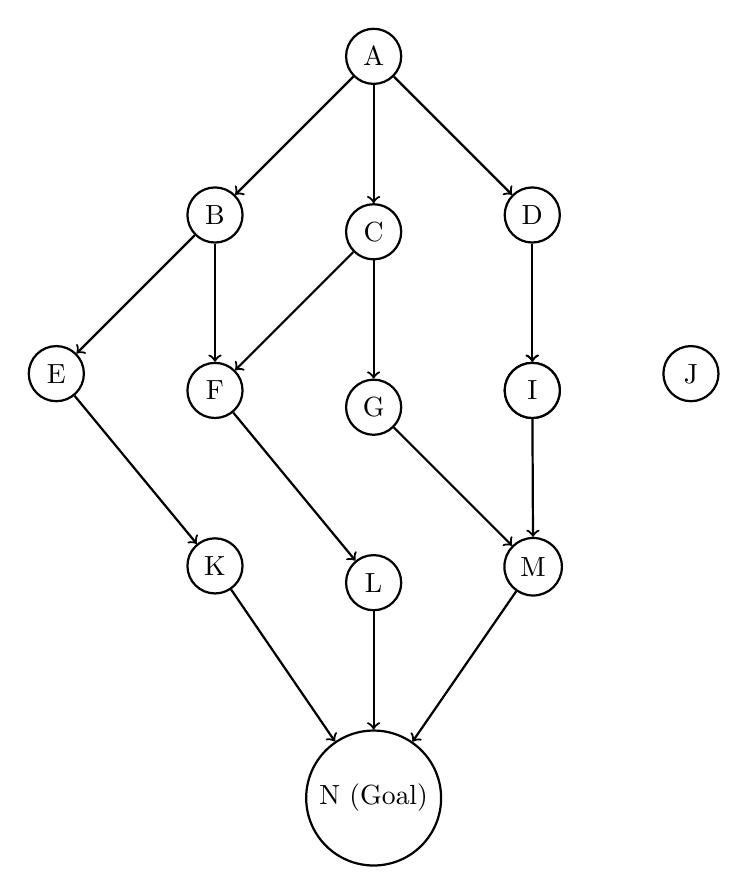
\begin{tikzpicture}[node distance=1.5cm and 1.5cm, roundnode/.style={circle, draw=black, fill=white, thick, minimum size=7mm}]
        % Nodes
        \node[roundnode] (A) {A};
        \node[roundnode] (B) [below left=of A] {B};
        \node[roundnode] (C) [below=of A] {C};
        \node[roundnode] (D) [below right=of A] {D};
        \node[roundnode] (E) [below left=of B] {E};
        \node[roundnode] (F) [below=of B] {F};
        \node[roundnode] (G) [below=of C] {G};
        \node[roundnode] (H) [below right=of C] {H};
        \node[roundnode] (I) [below=of D] {I};
        \node[roundnode] (J) [below right=of D] {J};
        \node[roundnode] (K) [below left=of G] {K};
        \node[roundnode] (L) [below=of G] {L};
        \node[roundnode] (M) [below right=of G] {M};
        \node[roundnode] (N) [below=of L] {N (Goal)};
    
        % Edges
        \draw[->, thick] (A) -- (B);
        \draw[->, thick] (A) -- (C);
        \draw[->, thick] (A) -- (D);
        \draw[->, thick] (B) -- (E);
        \draw[->, thick] (B) -- (F);
        \draw[->, thick] (C) -- (F);
        \draw[->, thick] (C) -- (G);
        \draw[->, thick] (D) -- (H);
        \draw[->, thick] (D) -- (I);
        \draw[->, thick] (E) -- (K);
        \draw[->, thick] (F) -- (L);
        \draw[->, thick] (G) -- (M);
        \draw[->, thick] (H) -- (M);
        \draw[->, thick] (K) -- (N);
        \draw[->, thick] (L) -- (N);
        \draw[->, thick] (M) -- (N);
    \end{tikzpicture}
    \end{center}
    
\subsection*{Misleading Heuristic:}
In highly connected graphs, even a reasonable heuristic can mislead A* into exploring unnecessary nodes. Below is a dense graph where A* fails to prioritize the shortest path efficiently.

A heuristic misaligned with the graph's geometry can guide A* in the wrong direction, causing it to explore irrelevant paths.

\subsection*{Heuristic Values}
The heuristic for the nodes is:
\[
h(A) = 10, \; h(B) = 8, \; h(C) = 1, \; h(D) = 8, \; h(E) = 1, \; h(F) = 5, \; h(G) = 0
\]

\subsection*{Problem}
- The heuristic overestimates costs in \( B \) and \( D \), guiding A* toward the path \( C \to E \to F \to G \), even though the shortest path is \( A \to B \to D \to F \to G \).
- The algorithm explores \( C \) and \( E \), wasting time on an unnecessary detour.

\begin{center}
    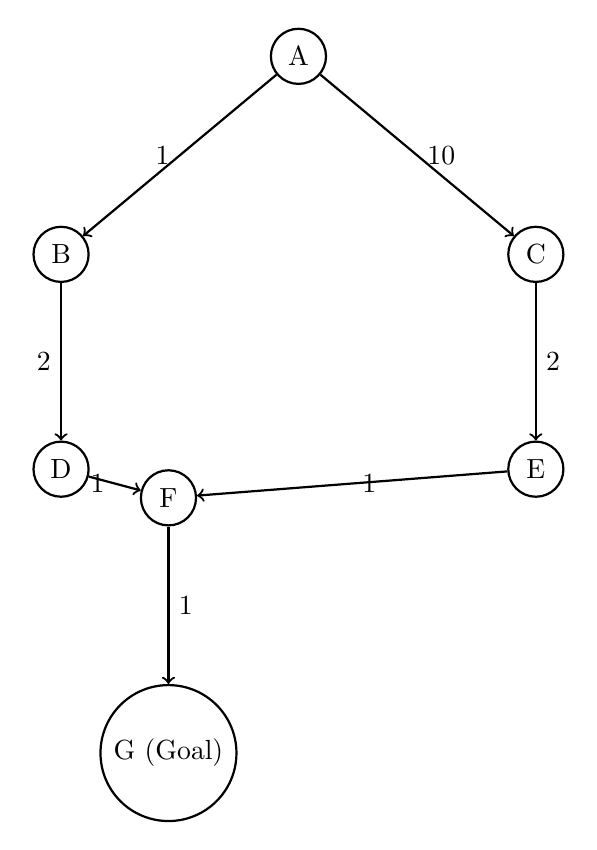
\begin{tikzpicture}[node distance=2cm and 2.5cm, roundnode/.style={circle, draw=black, fill=white, thick, minimum size=7mm}]
        % Nodes
        \node[roundnode] (A) {A};
        \node[roundnode] (B) [below left=of A] {B};
        \node[roundnode] (C) [below right=of A] {C};
        \node[roundnode] (D) [below=of B] {D};
        \node[roundnode] (E) [below=of C] {E};
        \node[roundnode] (F) [below=of D, right=1cm] {F};
        \node[roundnode] (G) [below=of F] {G (Goal)};
    
        % Edges
        \draw[->, thick] (A) -- (B) node[midway, left] {1};
        \draw[->, thick] (A) -- (C) node[midway, right] {10};
        \draw[->, thick] (B) -- (D) node[midway, left] {2};
        \draw[->, thick] (C) -- (E) node[midway, right] {2};
        \draw[->, thick] (D) -- (F) node[midway, left] {1};
        \draw[->, thick] (E) -- (F) node[midway, right] {1};
        \draw[->, thick] (F) -- (G) node[midway, right] {1};
    \end{tikzpicture}
    \end{center}
\subsection*{To improve efficiency:}
\begin{itemize}
    \item Use bidirectional A* to reduce the number of explored nodes. Start one search from the start and another from the goal, meeting in the middle.
    \item Ensure the heuristic is admissible (never overestimates the cost) and consistent (satisfies the triangle inequality).In cases like grids, use Manhattan or Euclidean distances to reflect actual geometry.
\end{itemize}


\end{document}
